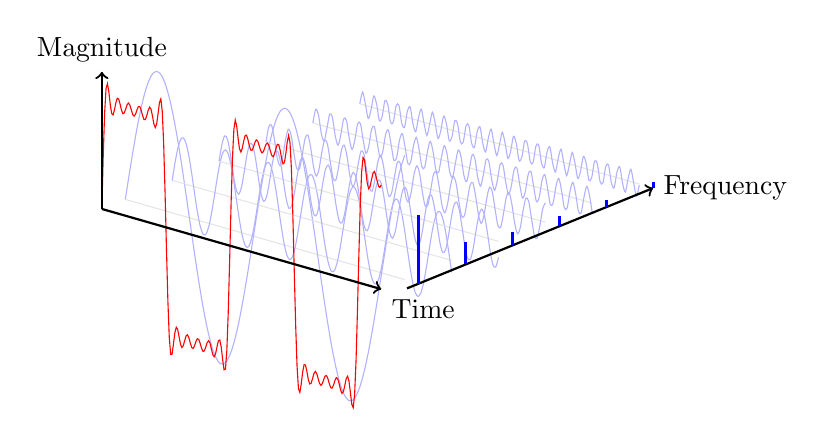
\begin{tikzpicture}

\begin{axis}[
    set layers=standard,
    domain=0:10,
    samples y=1,
    view={40}{20},
    hide axis,
    unit vector ratio*=2 4 2,
    xtick=\empty, ytick=\empty, ztick=\empty,
    clip=false
]
    \def\sumcurve{0}
    \pgfplotsinvokeforeach{0.5,1.5,...,5.5}{
        \draw [on layer=background, gray!20] (axis cs:0,#1,0) -- (axis cs:10,#1,0);
        \addplot3 [on layer=main, blue!30, smooth, samples=101]
            (x,#1,{2*sin(#1*x*(157))/(#1*2)});
        \addplot3 [on layer=axis foreground, very thick, blue,ycomb, samples=2]
            (10.5,#1,{1/(#1*2)});
        \xdef\sumcurve{\sumcurve + 2*sin(#1*x*(157))/(#1*2)}
    }
    \addplot3 [red, samples=200] (x,0,{\sumcurve});
    \draw[->,thick] (axis cs:0,0,0) -- (axis cs:0,0,2) node[above] {Magnitude};
    \draw[->,thick,on layer=axis foreground]  (axis cs:0,0,0) -- (axis cs:10,0,0) node[below right] {Time};
    \draw[->,thick] (axis cs:10.5,0.25,0) -- (axis cs:10.5,5.5,0) node[right] {Frequency};
\end{axis}

\end{tikzpicture}

%Local variables:
% coding: utf-8
% mode: text
% mode: rst
% End:
% vim: fileencoding=utf-8 filetype=tex :
